\chapter{Results}

\section{Learning on training data}

The first important thing to assess when working with neural networks is how they learn. Firstly do the model is really learning anything and improving the quality of its knowledge. This is first assessed in section \ref{section:isitlearning}. We also need to check the efficiency of pretraining our network on the CAT2000 dataset  \cite{DBLP:journals/corr/BorjiI15}. We do it in section \ref{section:pretrain} and section \ref{section:strategies}, comparing two learning processes and strategies. Finally we will see the importance of data-augmentation in section \ref{section:augmentation}.

\subsection{Is the network learning? (bad title to be changed)}\label{section:isitlearning}
\begin{figure}[ht!]
\centering
    \begin{tabular}{c@{\hspace{0.1cm}}c@{\hspace{0.3cm}}c@{\hspace{0.1cm}}c}
        
\includegraphics[width=0.22\linewidth]{./picsres/weights_14_1.png} &
        
\includegraphics[width=0.22\linewidth]{./picsres/weights_14_2.png} &
        
\includegraphics[width=0.215\linewidth]{./picsres/weights_14_vgg_2_1.png}&
         
\includegraphics[width=0.222\linewidth]{./picsres/weights_14_vgg_2_2.png}
    \end{tabular}
\centering
    \begin{tabular}{c@{\hspace{4.5cm}}c}
       {\small 14th conv layer  } & {\small VGG16  14th conv layer } 
     \end{tabular}
     \begin{tabular}{c@{\hspace{0.1cm}}c@{\hspace{0.3cm}}c@{\hspace{0.1cm}}c}
        
\includegraphics[width=0.22\linewidth]{./picsres/weights_19_2_1.png} &
        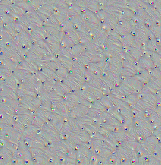
\includegraphics[width=0.22\linewidth]{./picsres/weights_19_2_2.png} &
        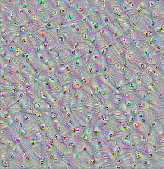
\includegraphics[width=0.215\linewidth]{./picsres/weights_19_vgg_2_1.png}&
         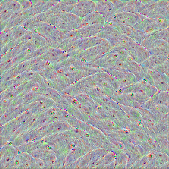
\includegraphics[width=0.222\linewidth]{./picsres/weights_19_vgg_2_2.png}
    \end{tabular}
     \begin{tabular}{c@{\hspace{5.5cm}}c}
              {\small 19th conv layer  } & {\small VGG16  19th conv layer }  

     \end{tabular}
    
    \caption{Comparison between the weights of our encoding network and VGG16}
    \label{fig:weights}
\end{figure}

When training a neural network, multiple ways can be used to see if the network is learning something and how does it learn it. The basic way would be to watch the loss progression and check if it is decreasing during the training. We can also check that the weights are not becoming random.
Figure \ref{fig:weights}, shows different filter/weights at various convolution layers. Their equivalent in the pretrained VGG are also displayed next to them. Those representation were produced by applying the forward pass of our network on a image with random values. By stopping at the desired layer and back-propagating from it while optimizing the image loss. The patterns formed are roughly the shape for which the learned filter is sensible.
We can see that our network has indeed learn something from our data as the weight have changed between our convolution layers and those of VGG. In particular for the 19th layer where we can see quite some difference between the two set of weights.

\subsection{Loss evolution}

\subsubsection{Loss evolution using pre-trained or not network}\label{section:pretrain}
We show in this section how pretraining our network on the visual attention dataset CAT2000 \cite{DBLP:journals/corr/BorjiI15} effect the overall training and our results. Figure \ref{fig:pretraining} show the effect of pretraining the network. We can see that without pretraining it the network is indeed learning but very slowly.
\begin{figure}[ht!]
    \centering
    \begin{tabular}{@{}c@{\hspace{0.1cm}}c@{\hspace{0.1cm}}c@{}}
        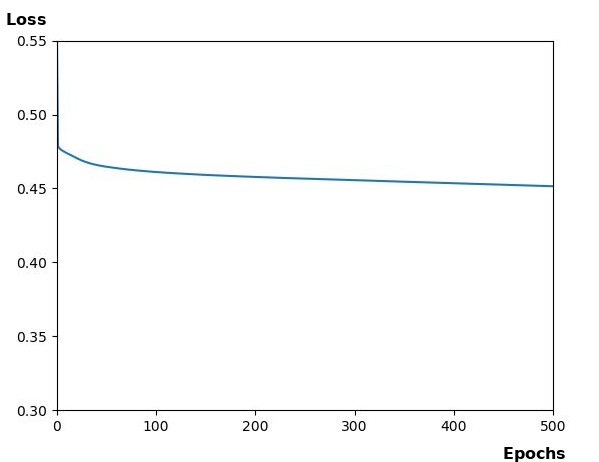
\includegraphics[width=0.518\linewidth]{./results/from_scratch_loss.png}& 
        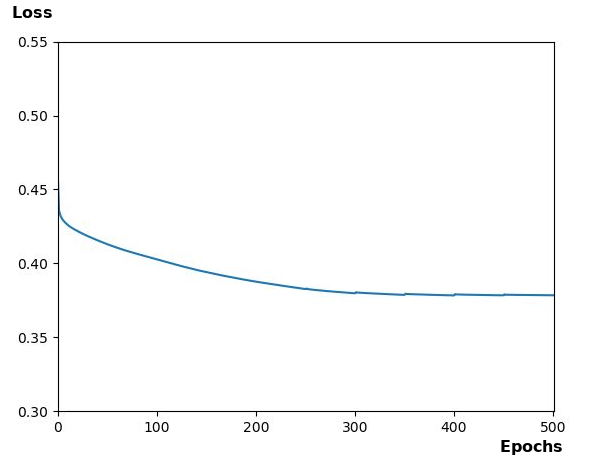
\includegraphics[width=0.505\linewidth]{./results/pretrained_loss.png}\\
        {\small Not pretrained network loss evolution} & {\small Pretrained network loss evolution} \\
       
    \end{tabular}
    \caption{Evolution of Loss for two networks, over 500 epochs. The first hasn't been pretrained while the second one has been pretrained on CAT2000 dataset \cite{DBLP:journals/corr/BorjiI15}}
    \label{fig:pretraining}
\end{figure}
Pretraining the network is effectively making the training process faster and improve results obtained. The explanation is coming from the decoder part of our network. Because we randomly initialized it it needs a lot of training to learn how to transform features extracted from the board to transform them into salient values. 
Training on the CAT2000 dataset becomes interested because of two main reasons : 
\begin{itemize}
    \item The features characterizing the CAT200 dataset are mainly the same as in the Imagenet dataset (faces,animals,plants etc..). And because our encoder part of the network is based in the imagenet pretrained VGG16, it doesn't need too much complementary training and can focus on training the decoder part. 
    \item The CAT2000 dataset offers a large amount of saliency map data. This allows our decoder part of the network to have enough resources to learn weights relevant for saliency map generation. 
\end{itemize}


\subsubsection{Effect of cyclical learning rate compared to standard decreasing learning rate}\label{section:strategies}

Figure \ref{fig:cyclicalr} shows the evolution of the loss during two training processes. The first one is an attempt using cyclical learning rate \cite{DBLP:journals/corr/Smith15a} and the second one decreasing the learning rate progressively. We can see that in the end, Cyclical learning rate  doesn't really affect the learning process in our case as we reach the same loss. 
\begin{figure}[ht!]
    \centering
    \begin{tabular}{@{}c@{\hspace{0.1cm}}c@{\hspace{0.1cm}}c@{}}
        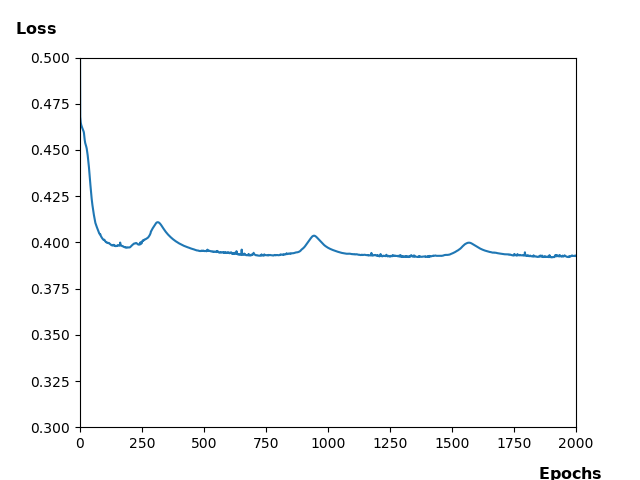
\includegraphics[width=0.50\linewidth]{./pics/cyclical_loss.png}& 
        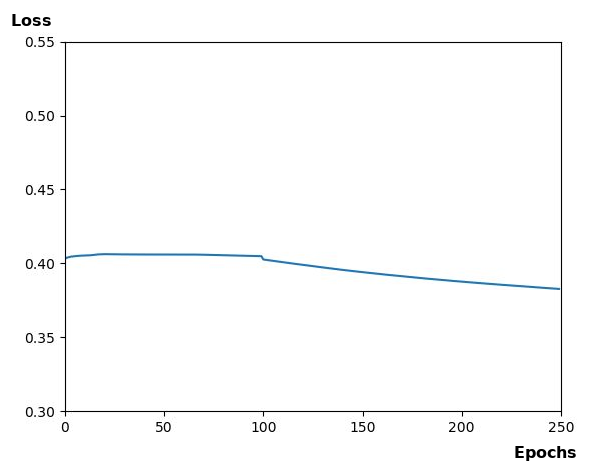
\includegraphics[width=0.50\linewidth]{./results/decreasing_lr.png}\\
        {\small  Using cyclical learning rate } & {\small Normal decreasing learning rate strategy} \\
       
    \end{tabular}
    \caption{Comparing two learning rate scheduling strategies}
    \label{fig:cyclicalr}
\end{figure}


However decreasing the learning rate is effectively reducing the loss faster than keeping the same learning rate for larger amounts of epochs. But after trying different learning rates and decreasing them or not, we end up finding that keeping a learning rate of 0.01 and training longer was an optimal strategy.

\subsection{Training our model on our dataset}
\begin{figure}[ht!]
    \centering
    \begin{tabular}{@{}c@{\hspace{0.1cm}}c@{}}
        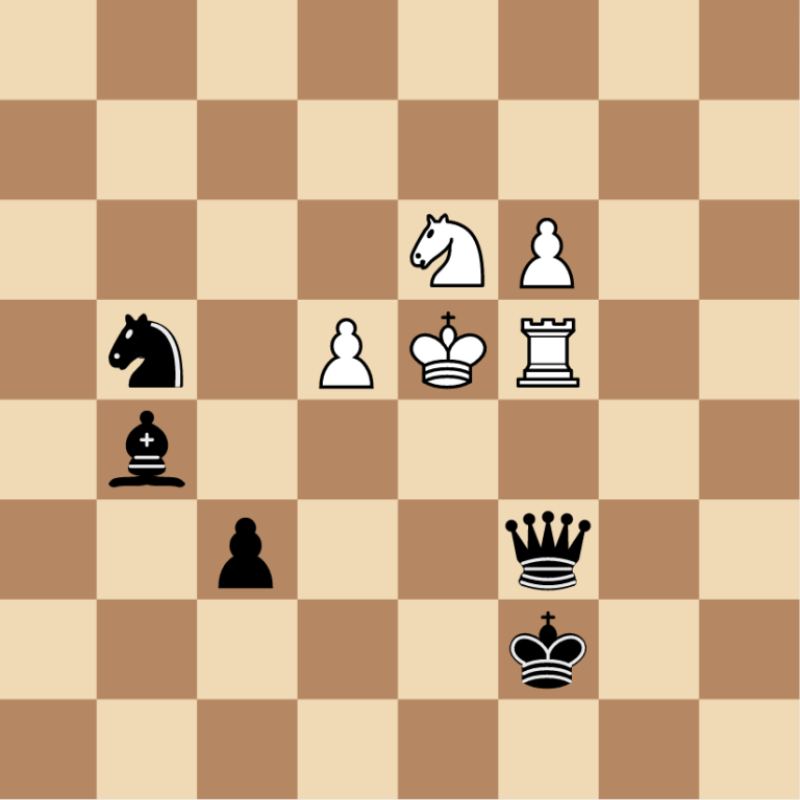
\includegraphics[width=0.22\linewidth]{./results/configIX.png}& 
        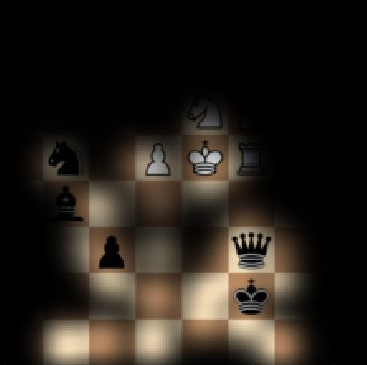
\includegraphics[width=0.225\linewidth]{./results/newonly_IX_res.png}\\
        
        {\small  Configuration reference} & {\small Predicted saliency} \\
    \end{tabular}
    \caption{Example of how a network only trained on our dataset performs}
    \label{fig:newonly}
\end{figure}
The idea behind this dataset wasn't to use it as our main source of training data, but rather to use it to pretrain our network and lead the network to learn pieces and moves. Hypothetically with enough training and diversified data, it would be possible for the network to learn what to play or the different possibilities for a lot of configurations. Because of the dataset size, we had to reduce the training time to few hundred of epochs instead of thousands. When we stopped the training, the loss was still slowly decreasing, but as figure \ref{fig:newonly} shows, we still have a bias related to the number of opening being too important as explained in \ref{section:descpnewdataset0}.



\subsection{Data augmentation results}\label{section:augmentation}
An other interesting thing to test was the usefulness of the data augmentation. For that we trained two models with no data augmentation other than cutting the board into four parts. The first one was pretrained on CAT2000 dataset\cite{DBLP:journals/corr/BorjiI15} and the second one on the dataset we created. Both were trained during 2000 epochs with a learning rate of 0.01. The results for those training on the test data are presented in figure \ref{fig:augment} with a model trained using data augmentation and pretrained on our dataset. The metrics used in figure \ref{fig:augment} are explained in section \ref{seq:metrics}.
\begin{figure}[ht!]
    \centering
\begin{tabular}{|c|c|c|c|c|c|}
  \hline
  Model/Metrics & LCC & SIM & NSS & AUC-Judd & AUC-Borji \\
  \hline
  V1.0 & 0.46 & 0.59 & 0.25 & 0.44 & 0.59 \\
  V2.0 & 0.67 & 0.69 & 0.24 & 0.63 & 0.73 \\
  V3.0 & 0.529 & 0.604 & 0.207 & 0.739 & 0.792\\
  \hline
\end{tabular}
 \caption{Models : \textbf{V1.0} No data augmentation pretrained on our dataset  \textbf{V2.0}
 No data augmentation pretrained on CAT2000 \textbf{V3.0} pretained on new data and then trained normally}
 \label{fig:augment}
\end{figure}

\begin{figure}[ht!]
    \centering
    \begin{tabular}{@{}c@{\hspace{0.1cm}}c@{\hspace{0.1cm}}}
        {\small Configuration 1} & {\small Configuration 2}&
        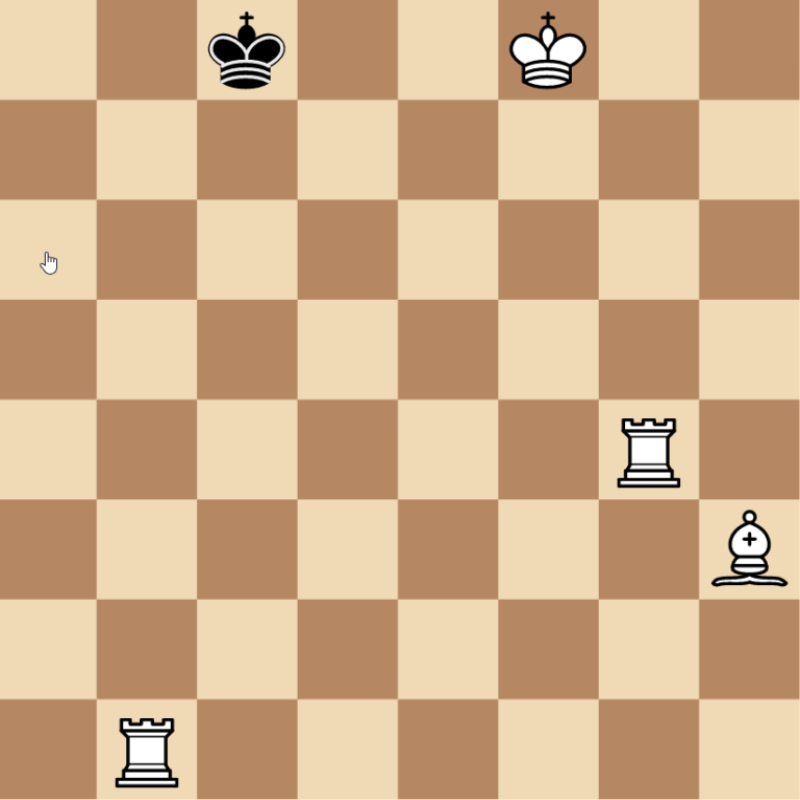
\includegraphics[width=0.22\linewidth]{./picsres/XVII.png}& 
        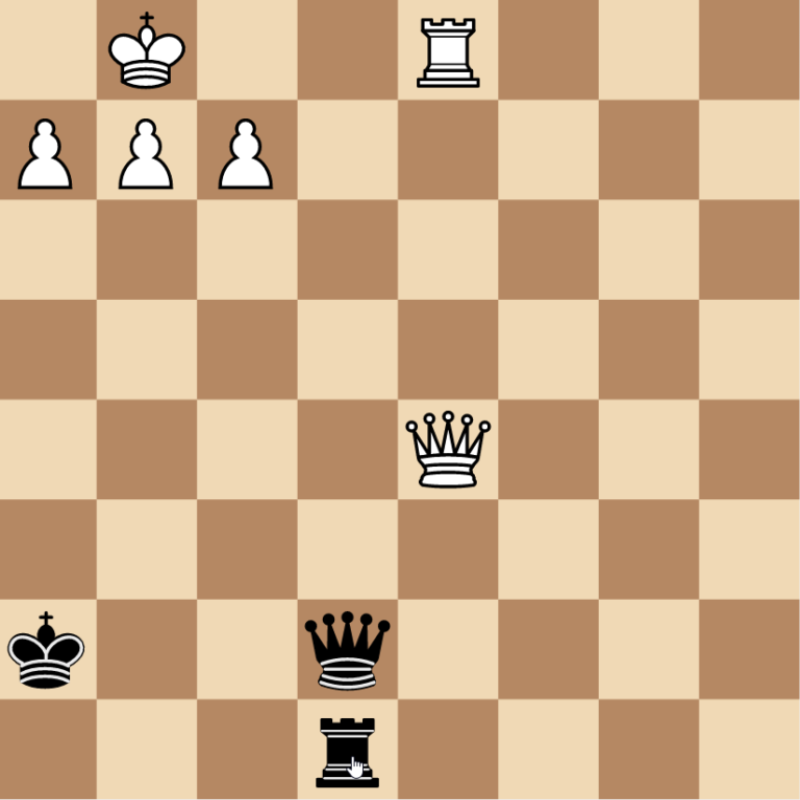
\includegraphics[width=0.22\linewidth]{./picsres/XXIX.png}\\
         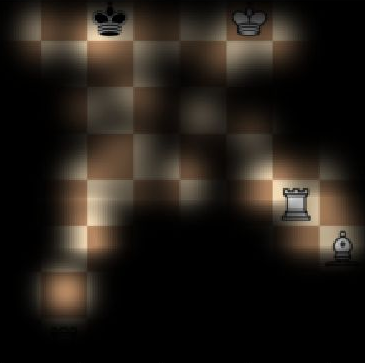
\includegraphics[width=0.22\linewidth]{./picsres/groundtruth_XVII.png}& 
        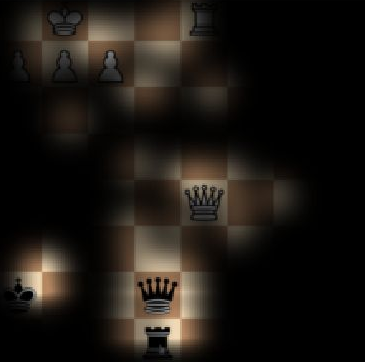
\includegraphics[width=0.22\linewidth]{./picsres/groundtruth_XXIX.png}\\
        
        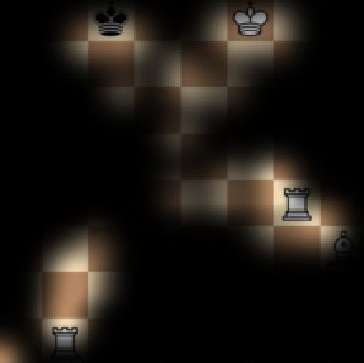
\includegraphics[width=0.22\linewidth]{./picsres/noaugment_old_XVII.png}& 
        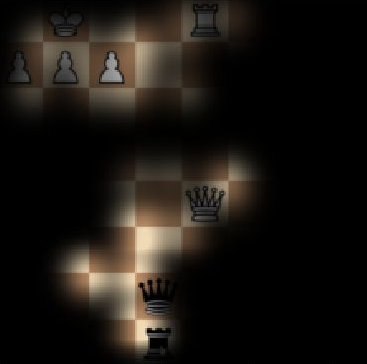
\includegraphics[width=0.22\linewidth]{./picsres/noaugment_old_XXIX.png}\\
         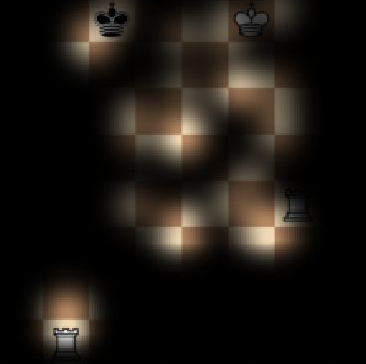
\includegraphics[width=0.22\linewidth]{./picsres/noaugment_new_XVII.png}& 
        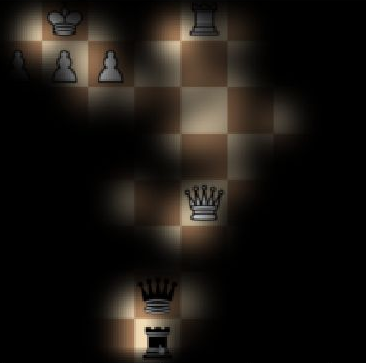
\includegraphics[width=0.22\linewidth]{./picsres/noaugment_new_XXIX.png}\\

    \end{tabular}
    \caption{The first line shows the configuration, the second line their saliency map groundtruth, the third line is the result obtained with \textbf{V2.0}, the fourth line are the results obtained using \textbf{V1.0} }
    \label{fig:augmentres}
\end{figure}
From figure \ref{fig:augment} we can see few things straight away. First when we do not use any data augmentation , pretraining the network on CAT2000 (\textbf{V1.0)}, improves the performances compare to the model pretrained on our dataset (\textbf{V3.0}). Metrics such as linear correlation, similarity and normalized scan path, reveal a stronger correlation between our results and the ground truth for the pretrained on CAT2000 network. Concerning results for the AUC metrics, the difference is even more important as for the V2.0 model, its AUC results  can be classified as nearly fair while V1.0 is closer to failure. V3.0 model shows better performances than the same model without data augmentation (V1.0), but is not as good than V2.0 for LCC, SIM and NSS. On the other hand V3.0 is behaving better for AUC metrics with fair/nearly good results.



Using these metrics is not an easy way to visualize how the model performs on real examples. For that we show in Figure \ref{fig:augmentres}, the output of our network for two test data. The first row represent the chess configuration and the ground truth superposed on it. The second are the results obtained with our two networks. We can see several differences betwee the two training strategies and the groundtruth. For the configuration XVII, the network trained on CAT2000, correctly focus on both kings, rooks and the bishop as the groundtruth does. On the other hand the other network doesn't show as much interest for the rook and bishop on the right side of the board. Concerning the XXIX configuration, both networks takes the black king out but correctly "see" the white king and rook and the white queen too. The black queen and rook which are the key to the check mate are salient for both networks. 

\section{Evaluation data}

\subsection{Comparing results for differently trained networks}
\begin{figure}[ht!]
    \centering
    \begin{tabular}{@{}c@{\hspace{0.1cm}}c@{\hspace{0.1cm}}}
            {\small Configuration 1 } & {\small Configuration 2}\\
        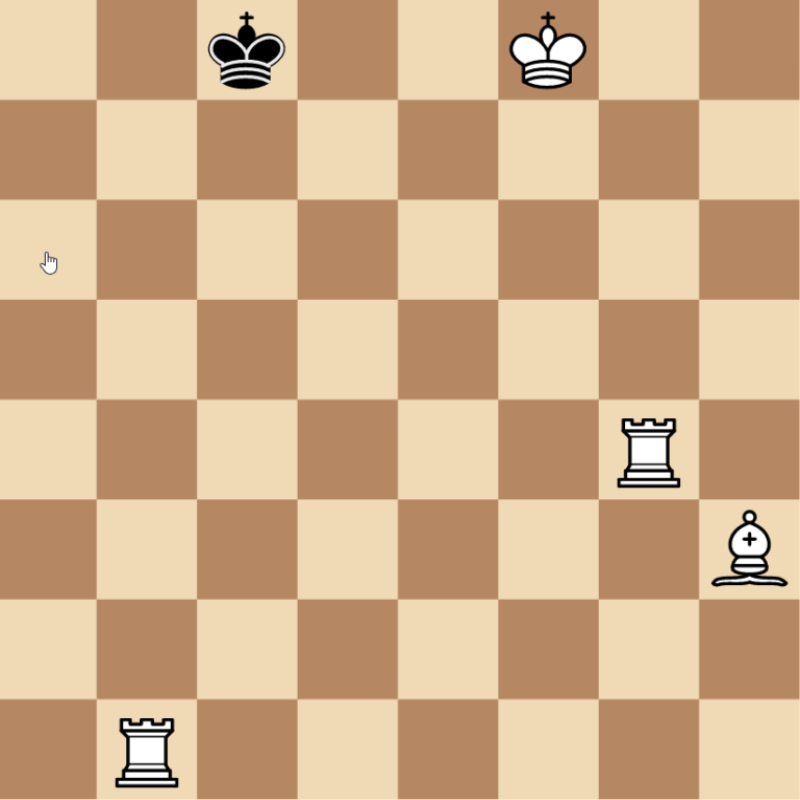
\includegraphics[width=0.28\linewidth]{./picsres/XVII.png}& 
        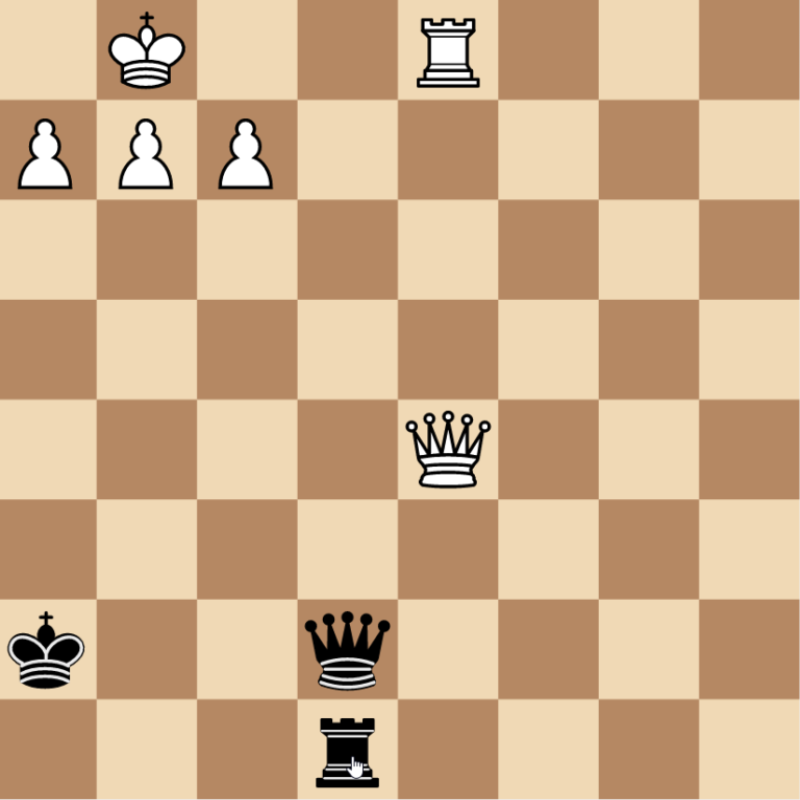
\includegraphics[width=0.28\linewidth]{./picsres/XXIX.png}\\
         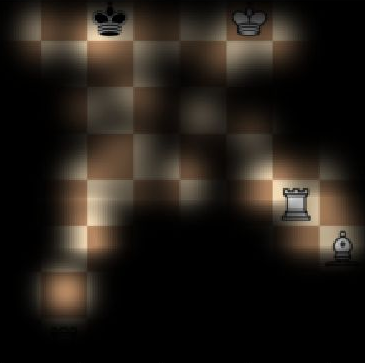
\includegraphics[width=0.28\linewidth]{./picsres/groundtruth_XVII.png}& 
        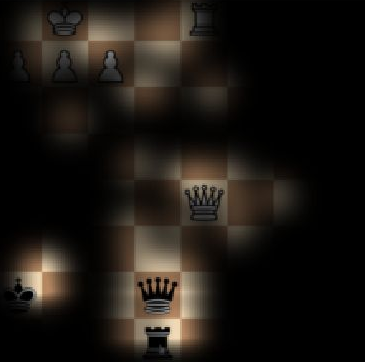
\includegraphics[width=0.28\linewidth]{./picsres/groundtruth_XXIX.png}\\
        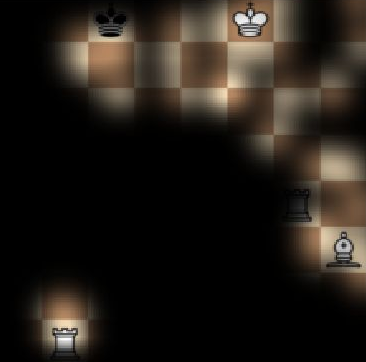
\includegraphics[width=0.28\linewidth]{./picsres/final_old_network_XVII.png}& 
        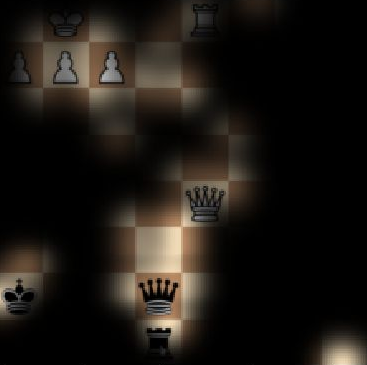
\includegraphics[width=0.28\linewidth]{./picsres/final_old_network_XXIX.png}\\
         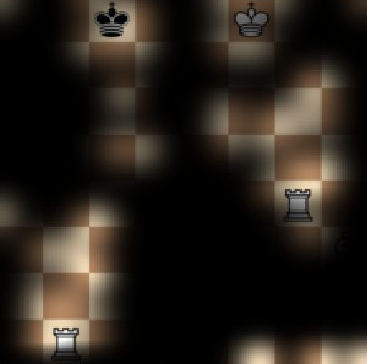
\includegraphics[width=0.28\linewidth]{./picsres/Final_new_XVII.png}& 
        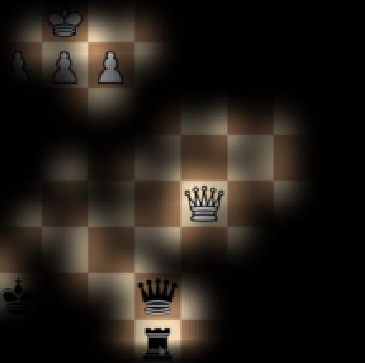
\includegraphics[width=0.28\linewidth]{./picsres/Final_new_XXIX.png}\\
        
    \end{tabular}
    \caption{Comparison of prediction for two differently trained models on the two testing configuration. The \textbf{first row} is our configuration. The \textbf{second row} the groundtruth from the users eye tracking data. The \textbf{third row} are the prediction from the network pretrained on CAT2000 dataset (\textbf{V1.0}) and \textbf{the last row} from the network pretrained on our dataset (\textbf{V3.0})}
    \label{fig:modelcomp}
\end{figure}

\begin{figure}[ht!]
    \centering
\begin{tabular}{|c|c|c|c|c|c|}
  \hline
  Model & LCC & SIM & NSS & AUC-Judd & AUC-Borji \\
  \hline
  V1.0 & 0.568 & 0.621 & 0.318 & 0.640 & 0.725 \\
  V2.0 & 0.316 & 0.490 & 0.094 & 0.573 & 0.673 \\
  V3.0 & 0.529 & 0.604 & 0.207 & 0.739 & 0.792\\
  \hline
\end{tabular}
 \caption{Models : \textbf{V1.0} pretrained and normally trained,\textbf{V2.0} trained only on new data, \textbf{V3.0} pretained on new data and then trained normally}
 \label{table:modelcomp}
\end{figure}

To evaluate our work we need to compare few models trained differently. Figure \ref{table:modelcomp}, shows how well three of our models perform.
The first one (V1.0) has been pretrained on CAT200 and trained normally on our augmented dataset. The second one (V2.0) has only been trained on our dataset. And finally the third (V3.0) one has been pretrained on our dataset and then trained normally on our augmented dataset. Concerning correlation metrics (LCC,SIM,NSS), the model pretrained on CAT2000 is performing better than the others. But for the AUC metrics, the model pretrained on our dataset, is the one showing better results.\\



Figure \ref{fig:modelcomp} is about comparing the output of V1.0 and V3.0 for configurations XVII and XXIX. Concerning the latter, the area of fixation of V3.0 is larger and more spread than V1.0, but doesn't include the white rook and not completely the black king. V3.0 is also considering more of the board for XVII than V1.0, and even too much, but excluding the white bishop. We can see that it "fixates" the bottom right part of the board while there is nothing here. It could come from that for our dataset there are a lot of castling happening on this side of the board. This pattern could have been learned by the network.


\subsection{Comparing performances for different training/validation cut}

In this section we are going to compare, how choosing differently the testing and training data among our augmented dataset affects the performances (for the same amount of training epochs and same learning rate of 0.01). Figure \ref{table:comptraintest} showcases these differences. We can see that the model \textbf{V3.*} is on average better concerning AUC metrics where it can be considered as fair, while \textbf{V1.*} is better for correlation metrics.

\begin{figure}[ht!]
    \centering
\begin{tabular}{|c|c|c|c|c|c|}
  \hline
  Model & LCC & SIM & NSS & AUC-Judd & AUC-Borji \\
  \hline
  V1.0 & 0.568 & 0.621 & 0.318 & 0.640 & 0.725 \\
  V3.0 & 0.529 & 0.604 & 0.207 & 0.739 & 0.792\\
  V1.1 & 0.549 & 0.619 & 0.331 & 0.719 & 0.770 \\
  V3.1 & 0.372 & 0.553 & 0.210 & 0.618 & 0.705 \\
  V1.2 & 0.807 & 0.722 & 0.295 & 0.554 & 0.659 \\
  V3.2 & 0.804 & 0.750 & 0.277 & 0.703 & 0.758 \\
  \hline
\end{tabular}
 \caption{Comparison between models trained on differently cut training/testing set. \textbf{V1.*} is pretrained on CAT2000 and \textbf{V3.*} on our dataset. \textbf{V*.0} is using the two last configurations as testing data. \textbf{V*.1} is using the two first configurations as testing data. And 
 \textbf{V*.2} is using the two third and fourth configurations as testing data.} 
 \label{table:comptraintest}
\end{figure}





\subsection{Prediction examples and analysis }\label{section:examples}
In this section we will see how our networks performed on various configurations.
To create those configuration we used the board editor from Liches \footnote{\url{https://en.lichess.org/editor}}
The first one \ref{fig:empty} is the simplest possible. An empty board, which in theory would return none or random short fixations on the board. We can see that this is the case for V3.0 where there are nearly no visual attention except on the top left corner, and very short and limited one all over the board (lighter purple). For V1.0, there are a lot more fixations in the bottom left corner and all over the top and right top corner.  
\begin{figure}[ht!]
    \centering
    \begin{tabular}{@{}c@{\hspace{0.1cm}}c@{\hspace{0.1cm}}c@{}}
        
\includegraphics[width=0.3\linewidth]{./results/empty.png}& 
        
\includegraphics[width=0.3\linewidth]{./results/res_empty.png}&
        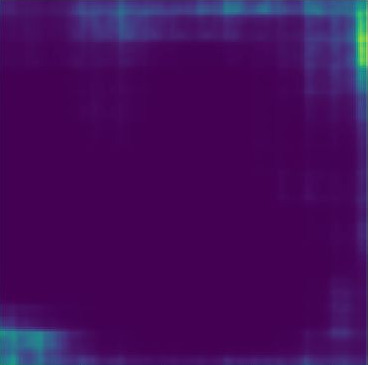
\includegraphics[width=0.3\linewidth]{./res2/empty_res_p.png}\\
        {\small An empty board  } & {\small V3.0 saliency map} &  {\small V1.0 saliency map}\\
       
    \end{tabular}
    \caption{The simplest configuration, and empty board}
    \label{fig:empty}
\end{figure}

The figure \ref{fig:queenking} depicts an other simple configuration. Here the black king is put in check by the white queen. We would expect fixations on the two pieces and on the vertical line between them showing their relation. V3.0 is close to  what we could expect but with some salient areas on the left part of the board. V1.0 on the other hand shows less saliency between the two pieces but some on the right part of the board.
\begin{figure}[ht!]
    \centering
    \begin{tabular}{@{}c@{\hspace{0.1cm}}c@{\hspace{0.1cm}}c@{}}
        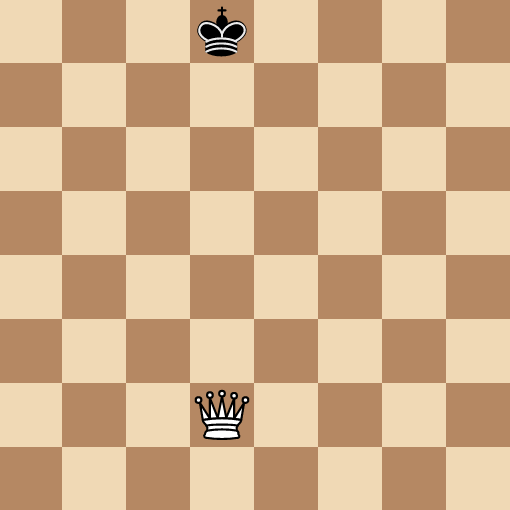
\includegraphics[width=0.3\linewidth]{./results/queen_and_king.png}& 
        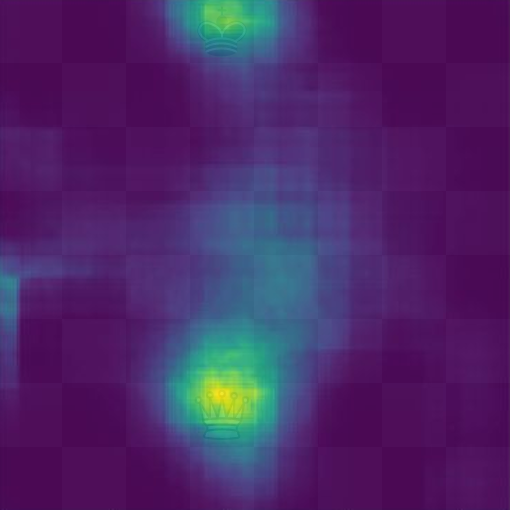
\includegraphics[width=0.3\linewidth]{./results/res2_sup.png}&
        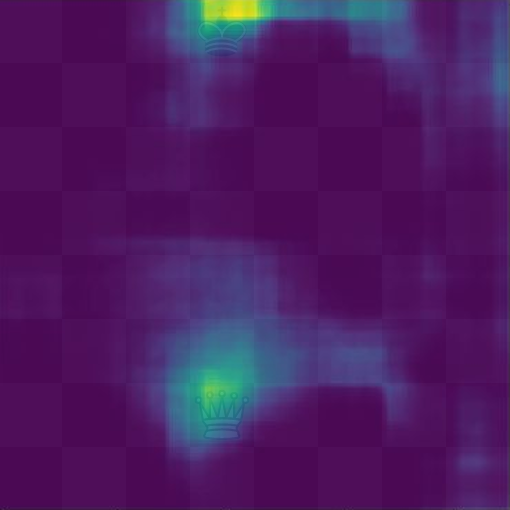
\includegraphics[width=0.3\linewidth]{./results/queen_and_king_res_p_sup.png}\\
        {\small An simple configuration  } & {\small V3.0 saliency map} &  {\small V1.0 saliency map}
    \end{tabular}
    \caption{An other simple configuration with only one king and its opponent queen}
    \label{fig:queenking}
\end{figure}

Now we try a more complicated configurations. Figure \ref{fig:withqueen}, is showing the white king in check. The only possibility is to move the king. The expected salient areas would be the white rooks, white king and  white queen and the black knight if we consider the king in check.
\begin{figure}[ht!]
    \centering
    \begin{tabular}{@{}c@{\hspace{0.1cm}}c@{\hspace{0.1cm}}c@{}}
        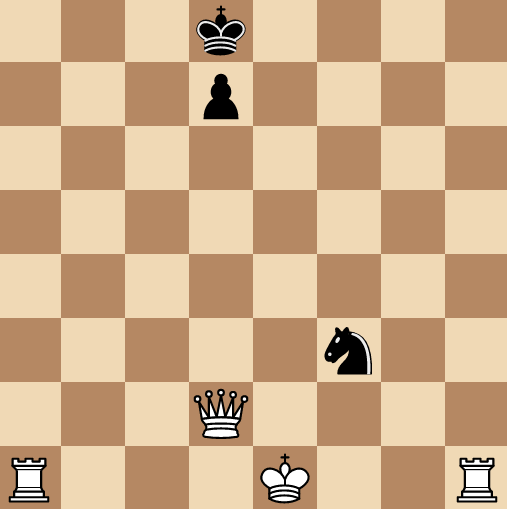
\includegraphics[width=0.3\linewidth]{./results/check_config1.png}& 
        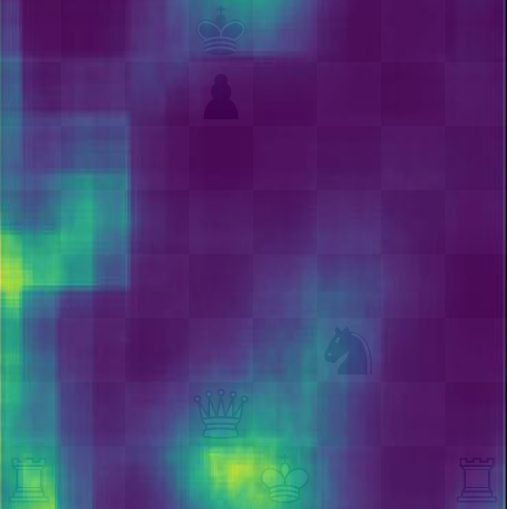
\includegraphics[width=0.3\linewidth]{./results/res_config1_sup.png}& 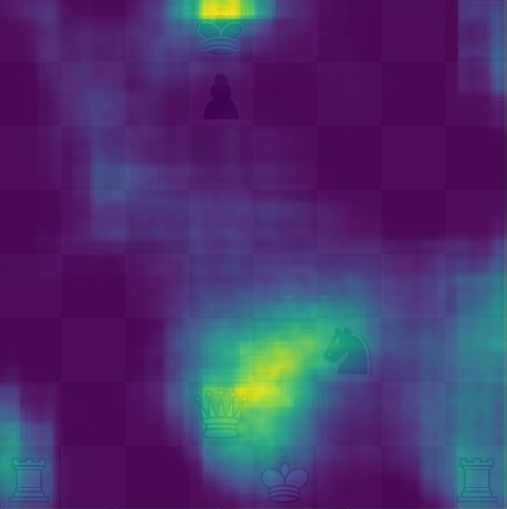
\includegraphics[width=0.3\linewidth]{./results/config1_res_sup.png}\\
        {\small An simple configuration  } & {\small V3.0 saliency map} &  {\small V1.0 saliency map}
       
    \end{tabular}
    \caption{A bit more complicated configuration. The white king is in check}
    \label{fig:withqueen}
\end{figure}
 If we don't know the check rule, the white queen diagonal and rooks vertical lines would be salient as they can attack the enemy king this way.
Here V3.0 considers all pieces and the position from where the queen would put the enemy king in check. But rooks verticals are not considered. V1.0 is considering moving the right rook upward and put the king in check more salient with the black knight.\\




\begin{figure}[ht!]
    \centering
    \begin{tabular}{@{}c@{\hspace{0.1cm}}c@{\hspace{0.1cm}}c@{}}
        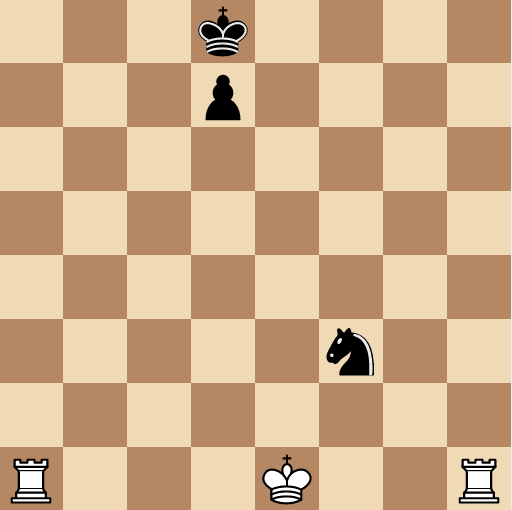
\includegraphics[width=0.3\linewidth]{./results/without_queen.png}& 
        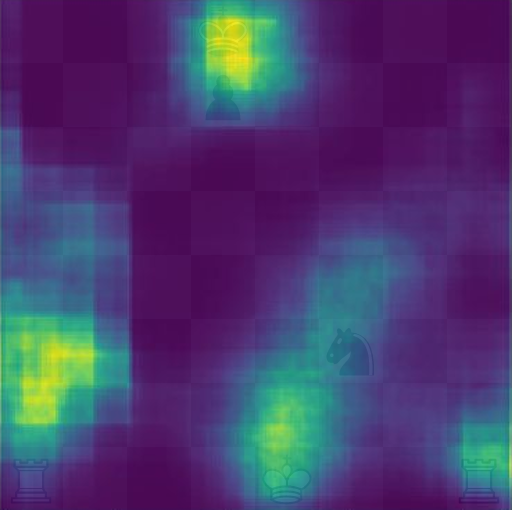
\includegraphics[width=0.3\linewidth]{./results/without_queen_res_new_sup.png}& 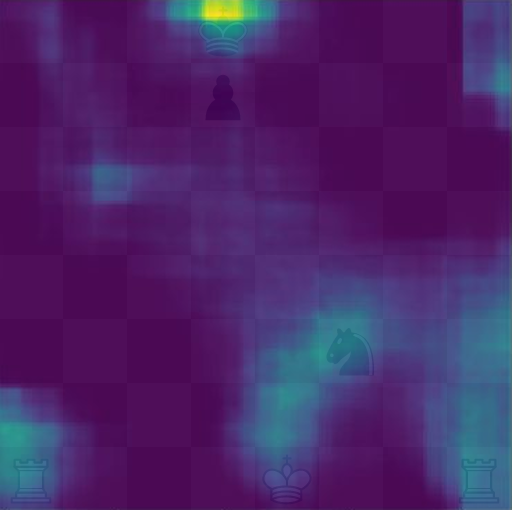
\includegraphics[width=0.3\linewidth]{./results/without_queen_res_old_sup.png}\\
        {\small An simple configuration  } & {\small V3.0 saliency map} &  {\small V1.0 saliency map}
       
    \end{tabular}
    \caption{Same configuration as in \ref{fig:withqueen} but without the queen}
    \label{fig:withoutqueen}
\end{figure}

Now we can try to remove the queen from previous configuration \ref{fig:withqueen}, which gives us the configuration \ref{fig:withoutqueen}.

We should expect the saliency to be the same as previously , but without the queen area and its diagonal, with a stronger saliency between the white king an the black knight. V3.0 is verifying part of those expectation, as the link between knight and king is stronger but strangely some salient area in front of the left rook appears stronger than previously. V1.0 on the other hand has reduced the overall saliency except for the enemy king.

\begin{figure}[ht!]
    \centering
    \begin{tabular}{@{}c@{\hspace{0.1cm}}c@{\hspace{0.1cm}}c@{}}
        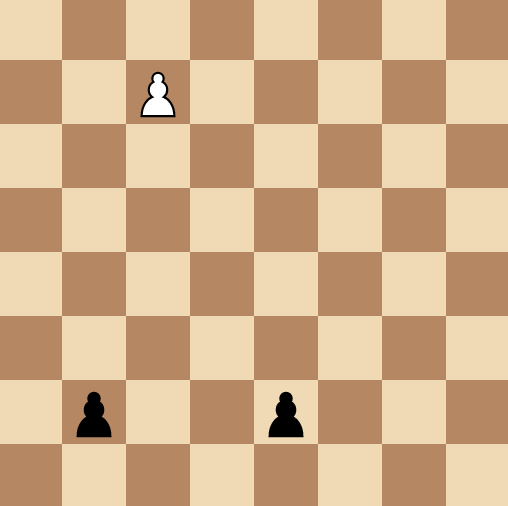
\includegraphics[width=0.3\linewidth]{./results/only_pawns.png}& 
        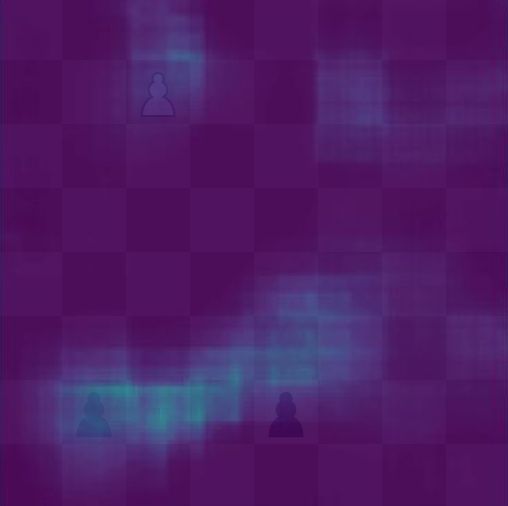
\includegraphics[width=0.3\linewidth]{./results/pawns-res_sup.png}& 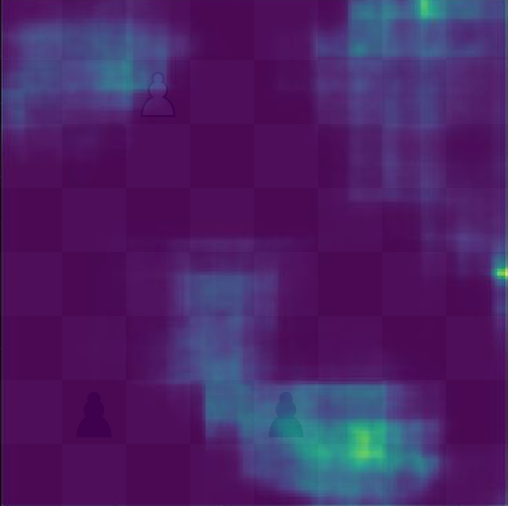
\includegraphics[width=0.3\linewidth]{./results/pawns-res_p_sup.png}\\
        {\small An simple configuration  } & {\small V3.0 saliency map} &  {\small V1.0 saliency map}
       
    \end{tabular}
    \caption{A configuration with only 3 pawns}
    \label{fig:pawns}
\end{figure}
The configuration presented in \ref{fig:pawns} is quite simple as there are only three pawns. We expect to have the three pawns salient, but with a small saliency as they don't really have any purpose. Here V3.0 is corresponding to our expectation even adding the area in front of our right black pawn as it is a recurrently played piece. V1.0 however considers the cells in front of the right pawn but also some area on the right behind it and on the top right corner.

\begin{figure}[ht!]
    \centering
    \begin{tabular}{@{}c@{\hspace{0.1cm}}c@{\hspace{0.1cm}}c@{}}
        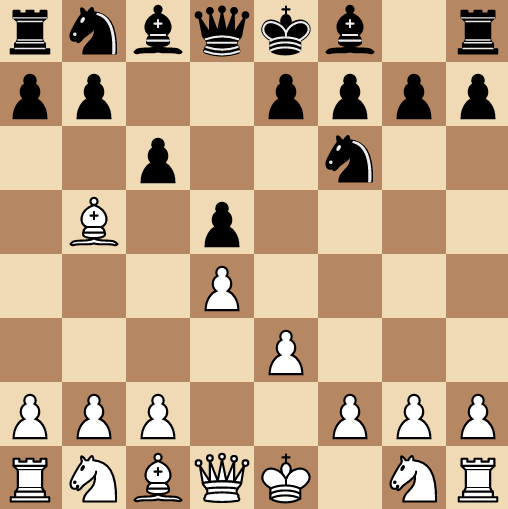
\includegraphics[width=0.30\linewidth]{./res2/opening.png}& 
        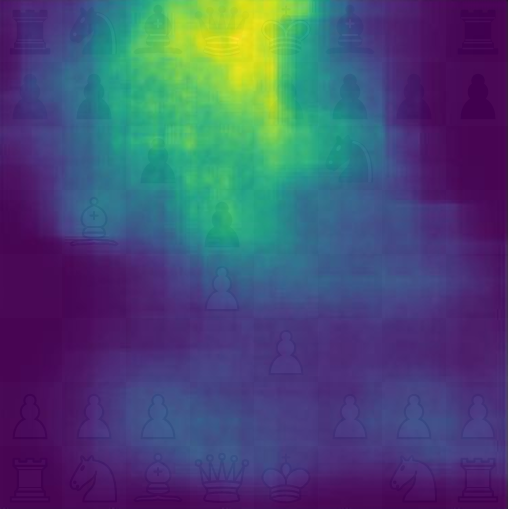
\includegraphics[width=0.30\linewidth]{./res2/pretrained_new_opening_res_sup.png} &
        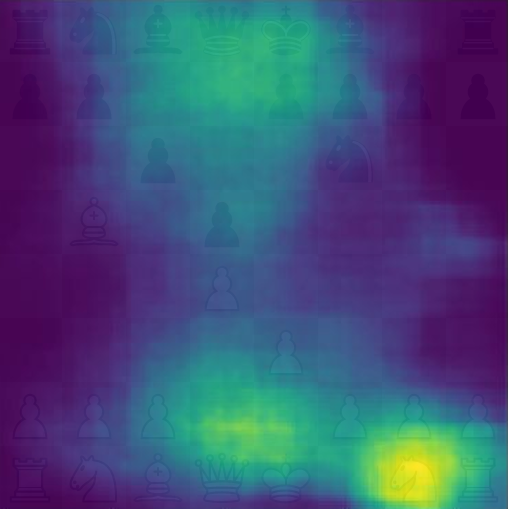
\includegraphics[width=0.30\linewidth]{./res2/pretrained_old_opening_res_sup.png}\\
        {\small An simple configuration  } & {\small V3.0 saliency map} &  {\small V1.0 saliency map}
       
    \end{tabular}
    \caption{An opening with a bishop in danger}
    \label{fig:opening}
\end{figure}
Figure \ref{fig:opening} is different from the others, considering the number of pieces. Here the white bishop in B5 is in danger because of the black pawn in C6. The logic way to do is to move the bishop either back or on the left. V3.0  shows the area surrounding the king/queen of the enemy and including the white bishop (the king was in check the round before). V1.0 consider the bottom right region (castling area) to be more salient than the rest and doesn't include the white bishop.

\begin{figure}[ht!]
    \centering
    \begin{tabular}{@{}c@{\hspace{0.1cm}}c@{\hspace{0.1cm}}c@{}}
        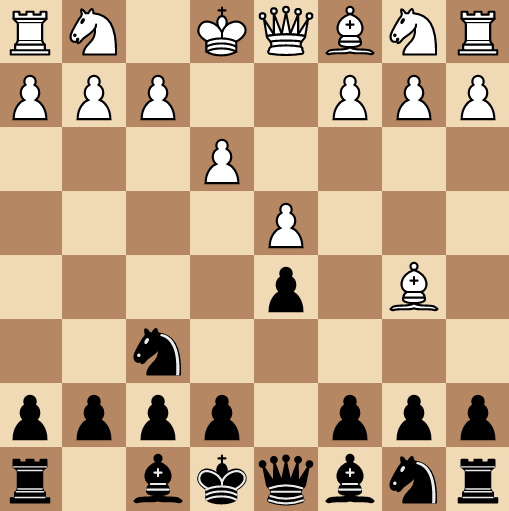
\includegraphics[width=0.30\linewidth]{./res2/opening_black_side.png}& 
        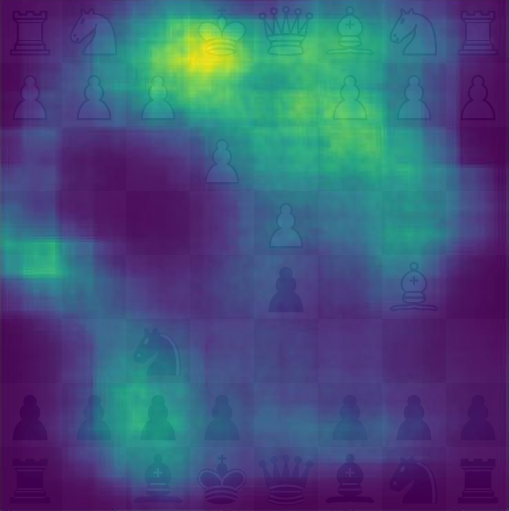
\includegraphics[width=0.30\linewidth]{./res2/opening_black_side_new_sup.png} &
        \includegraphics[width=0.30\linewidth]{./res2/opening_black_side_old_sup.png}\\
        {\small An simple configuration  } & {\small V3.0 saliency map} &  {\small V1.0 saliency map}
       
    \end{tabular}
    \caption{Same opening as \ref{fig:opening}, but one round before, on the black side}
    \label{fig:opening_black_side}
\end{figure}
Reverting the figure \ref{fig:opening} to see the game from the black perspective one round before, gives us figure \ref{fig:opening_black_side}. Here V3.0 doesn't seem to taking in consideration the bishop putting the king in check, but is showing the black bishop on white cells which can be put in B5 to put the queen in danger. V1.0 consider most of the board with an accent on the surroundings of the black queen and white king, including the dangerous white bishop.


\begin{figure}[ht!]
    \centering
    \begin{tabular}{@{}c@{\hspace{0.1cm}}c@{\hspace{0.1cm}}c@{}}
        \includegraphics[width=0.30\linewidth]{./results/knight_and_pawns.png}& 
        \includegraphics[width=0.30\linewidth]{./results/knight_and_pawns_res_new_sup.png} &
        \includegraphics[width=0.30\linewidth]{./results/knight_and_pawns_res_old_sup.png}\\
        {\small An simple configuration  } & {\small V3.0 saliency map} &  {\small V1.0 saliency map}
       
    \end{tabular}
    \caption{A choice for a knight}
    \label{fig:choice}
\end{figure}
This last configuration (Figure \ref{fig:choice} ) shows a white knight having two choices. It can either kill the pawn and be killed by the queen or kill the queen and kill the pawn next round. We would expect the area around the three pieces to be salient as well as the space between them. V3.0 once more corresponds to our assumptions choosing the queen to be more salient with the knight. V1.0 chooses also the queen and the knight but add salient areas a bit everywhere on the board too. 